\chapter{Second phase formation in Bayer alumina}

\section{Introduction}
Second phases such as spinel \cite{Zuo2013}, calcium hexaluminate \cite{Cinibulk1995}, and $\beta$-Al$_{2}$O$_{3}$ \cite{Duncan1969a}, are known to form during the sintering of Bayer alumina as a result of dopants and impurities such as MgO, CaO, and Na$_{2}$O. For Bayer aluminas, $\beta$-Al$_{2}$O$_{3}$ (Na$_{2}$O$\cdot$11Al$_{2}$O$_{3}$) is of particular interest because Na$_{2}$O is present up to a few hundred ppm. Rankin and Merwin \cite{Rankin1916} were the first to observe the formation of a new alumina phase in the high Al$_{2}$O$_{3}$ region in the system CaO-Al$_{2}$O$_{3}$-MgO. They believed it was an allotropic modification of Al$_{2}$O$_{3}$, and named it $\beta$-Al$_{2}$O$_{3}$. However, later work clarified that there is a relation between the alkali content in the Al$_{2}$O$_{3}$ and the formation of $\beta$-Al$_{2}$O$_{3}$ \cite{Stillwell1926}, and that $\beta$-Al$_{2}$O$_{3}$ is an alkali aluminate, rather than an allotropic form of Al$_{2}$O$_{3}$ \cite{Vries1969}. Ridgway et al. \cite{Ridgway1936} reported that the Na$_{2}$O content in Bayer process alumina is sufficient to form $\beta$-Al$_{2}$O$_{3}$. Four types of beta aluminas have been reported; two of them, $\beta$-Al$_{2}$O$_{3}$ (Na$_{2}$O$\cdot$11Al$_{2}$O$_{3}$) and $\beta$"-Al$_{2}$O$_{3}$ (Na$_{2}$O$\cdot$5Al$_{2}$O$_{3}$), form in the binary system Na$_{2}$O-Al$_{2}$O$_{3}$ and these phases can dissolve up to 2.5 and 5 wt.\% MgO, respectively \cite{Kummer1972a}. The other two beta aluminas, $\beta$'''-Al$_{2}$O$_{3}$ and $\beta$''''-Al$_{2}$O$_{3}$ are found at higher MgO concentrations in the ternary system Na$_{2}$O-Al$_{2}$O$_{3}$-MgO \cite{Kummer1972a,Stevens1984}. For completeness it should be mentioned that the existence of a $\beta$'-Al$_{2}$O$_{3}$ (Na$_{2}$O$\cdot$7Al$_{2}$O$_{3}$) has been reported, but subsequent literature is in agreement that $\beta$'-Al$_{2}$O$_{3}$ is actually $\beta$-Al$_{2}$O$_{3}$ with excess Na$_{2}$O \cite{Kummer1972a,Stevens1984}.

The fabrication and stability of $\beta$-Al$_{2}$O$_{3}$ powder has been extensively reported for the fabrication of the solid electrolyte in Na-S batteries. Most $\beta$-Al$_{2}$O$_{3}$ powder synthesis studies use sodium carbonate and alumina \cite{Vries1969,Kummer1972a,Ray1975}, which when heated to 1100$^{\circ}$C leads to the formation of $\beta$"-Al$_{2}$O$_{3}$ and decomposes to $\beta$-Al$_{2}$O$_{3}$ and NaAlO$_{2}$ at >1500$^{\circ}$C. The equilibrium vapor pressure of Na$_{2}$O over $\beta$-Al$_{2}$O$_{3}$ has been reported to be "appreciable" at >1400$^{\circ}$C \cite{Kummer1972a}, and thus $\beta$-Al$_{2}$O$_{3}$ can decompose to $\alpha$-Al$_{2}$O$_{3}$ by volatilization of Na$_{2}$O. Gallup \cite{Gallup1935} investigated the high temperature stability of $\beta$-Al$_{2}$O$_{3}$ under different atmospheres and reported that $\beta$-Al$_{2}$O$_{3}$ can transform to $\alpha$-Al$_{2}$O$_{3}$ at 1300$^{\circ}$C when heated in hydrogen or vacuum atmosphere. Interestingly, $\beta$-Al$_{2}$O$_{3}$ did not convert to $\alpha$-Al$_{2}$O$_{3}$ after heating for 1 h at 1500$^{\circ}$C in air, but fully converted when heated for 10 min at 1600$^{\circ}$C. 

There has been little study of $\beta$-Al$_{2}$O$_{3}$ formation in $\alpha$-Al$_{2}$O$_{3}$ ceramics even though $\beta$-Al$_{2}$O$_{3}$ grains in $\alpha$-Al$_{2}$O$_{3}$ ceramics can greatly impact electrical and structural properties. Duncan and Creyke \cite{Duncan1969a} investigated the formation and stability of $\beta$-Al$_{2}$O$_{3}$ in $\alpha$-Al$_{2}$O$_{3}$ ceramics and reported that $\beta$-Al$_{2}$O$_{3}$ forms at Na$_{2}$O concentrations as low as 0.04 wt.\% if 0.25 wt.\% MgO is present. An increase in $\beta$-Al$_{2}$O$_{3}$ content was observed for powders with higher Na$_{2}$O and MgO concentrations. They showed by electron-probe microanalysis that there is a higher concentration of Na$_{2}$O and MgO in the $\beta$-Al$_{2}$O$_{3}$ grains, and that $\beta$-Al$_{2}$O$_{3}$ is stable in dense $\alpha$-Al$_{2}$O$_{3}$ samples (24 mm diameter x 7 mm thick) up to 1650$^{\circ}$C in static air. In flowing air, however, $\beta$-Al$_{2}$O$_{3}$ decomposes to $\alpha$-Al$_{2}$O$_{3}$ even in the center of the sample.

To date, there is no systematic study on the effect of Na$_{2}$O and SiO$_{2}$ on the formation of $\beta$-Al$_{2}$O$_{3}$ during the sintering of MgO-doped Bayer alumina powders. The goals of this work are to identify the stages and mechanisms of $\beta$-Al$_{2}$O$_{3}$ formation in $\alpha$-Al$_{2}$O$_{3}$ ceramics during sintering and to determine how specific chemistries affect $\beta$-Al$_{2}$O$_{3}$ formation.

\section{Experimental}
A 380 ppm MgO-doped Bayer alumina (99.92\% pure, Almatis, Inc., Leetsdale, PA, USA) was chosen to investigate the formation of $\beta$-Al$_{2}$O$_{3}$. Physical and chemical characteristics of the powder are shown in Table \ref{Ch5-table:table1}. The powder was doped with up to 1000 ppm Na$_{2}$O and 1000 ppm SiO$_{2}$ using sodium acetate (NaC$_{2}$H$_{3}$O$_{2}$$\cdot$3H$_{2}$O, ACS grade, BDH, West Chester, PA), and TEOS (Si(OC$_{2}$H$_{5}$)$_{4}$, 98\%, Aldrich Chemical Company, Inc., Milwaukee, WI), respectively. The detailed doping procedures were described in previous chapters. After drying the powders were sieved to -106 $\mu$m, dry pressed at 170 MPa, and subsequently cold isostatically pressed at 200 MPa (CIP, Autoclave Engineers, Erie, PA) to form $\sim$3 mm tall cylindrical samples with 6 mm and 12.7 mm in diameter. The samples were sintered in a box furnace at 10$^{\circ}$C/min to 1200$^{\circ}$C and then at 5$^{\circ}$C/min to the final temperature between 1450$^{\circ}$C and 1600$^{\circ}$C, followed by a hold time of up to 8 h. The sintered samples were ground to half their initial height and polished to a surface finish of 1 $\mu$m. The crystal structure of the second phase was identified by x-ray diffraction (XRD, X'Pert Pro MPD, PANalytical B.V., The Netherlands) using Cu K$_{\alpha}$ radiation. The concentration of $\beta$-Al$_{2}$O$_{3}$ grains was determined on a minimum area of 0.1 mm$^{2}$ from the center of the samples using scanning electron microscopy (SEM, Phenom ProX; Phenom-World B.V., Eindhoven, The Netherlands). SEM micrographs obtained from backscattered electrons were used to detect $\beta$-Al$_{2}$O$_{3}$ grains. The contrast, brightness, and sharpness of the obtained SEM images were adjusted to improve the visibility of the second phases. The size of the $\beta$-Al$_{2}$O$_{3}$ grains was measured from the SEM images (length and thickness) and an area fraction was estimated. Considering the stereology of randomly oriented, platelet shaped $\beta$-Al$_{2}$O$_{3}$ grains \cite{Underwood1972} the estimated area fraction was assumed to be equal to the volume fraction of $\beta$-Al$_{2}$O$_{3}$ in the samples. The chemical composition of the second phase was determined by energy dispersive x-ray spectroscopy (EDS, Phenom ProX; Phenom-World B.V., Eindhoven, The Netherlands). Note that the samples for SEM analysis were not coated with a conducting material since such coatings can obscure second phases. 

\section{Results}
Figure \ref{Ch5-figure:Figure1} shows an example of second phases observed in sintered Bayer alumina. The second phase grains are platelet shaped, as evident from the high aspect ratio of the second phase grains. Initial studies showed that the detection of this second phase is challenging because no second phase grains are observed after thermal etching and in unetched samples the second phase grains can only be observed if a backscattered electron detector is used, as seen in Figure \ref{Ch5-figure:Figure1}. Furthermore, coatings that are typically applied on insulating samples to achieve sufficient electrical conductivity for SEM analysis can obscure the second phase grains, and therefore the samples were not coated.

Figure \ref{Ch5-figure:Figure2} shows the XRD pattern of a 99\% dense Bayer alumina sample doped with 1060 ppm Na$_{2}$O and 582 ppm SiO$_{2}$ and sintered at 1525$^{\circ}$C for 5 h. The small amount of second phase was indexed and identified as $\beta$-Al$_{2}$O$_{3}$ (PDF number: 98-001-2968). The estimated amount of $\beta$-Al$_{2}$O$_{3}$ from Rietveld analysis is 0.6 wt.\% and EDS analysis reveals that the $\beta$-Al$_{2}$O$_{3}$ grains contain higher concentrations of MgO and Na$_{2}$O relative to the surrounding matrix. As noted earlier, the Al$_{2}$O$_{3}$-Na$_{2}$O-MgO phase diagram shows that $\beta$-Al$_{2}$O$_{3}$ can dissolve up to 2.5 wt\% MgO \cite{Kummer1972a}.

Samples were heated for up to 8 h at 1525$^{\circ}$C to determine when $\beta$-Al$_{2}$O$_{3}$ forms during sintering and Figure \ref{Ch5-figure:Figure3} shows micrographs of MgO-doped Bayer alumina samples doped with 560 ppm Na$_{2}$O and 82 ppm SiO$_{2}$ after heating for 0 h, 1 h, and 8 h. The relative densities of the samples were 92\%, 97\%, and 99\%, respectively. It can be seen that the $\beta$-Al$_{2}$O$_{3}$ grains are 4 - 10 $\mu$m long and their size does not change as a function of sintering time. However the number of $\beta$-Al$_{2}$O$_{3}$ grains increases with increasing sintering time. To estimate how the amount of $\beta$-Al$_{2}$O$_{3}$ changes as a function of sintering time and powder chemistry the number density of $\beta$-Al$_{2}$O$_{3}$ grains per unit area was determined. 

The kinetics of $\beta$-Al$_{2}$O$_{3}$ formation in MgO-doped Bayer alumina is shown in Figure \ref{Ch5-figure:Figure4} as a function of powder chemistry. Most $\beta$-Al$_{2}$O$_{3}$ grains form within the first hour at 1525$^{\circ}$C, and after that the number density of $\beta$-Al$_{2}$O$_{3}$ grains does not change as a function of hold time for all chemistries. For example, samples with 560 ppm Na$_{2}$O and 82 ppm SiO$_{2}$ form $\sim$320 $\beta$-Al$_{2}$O$_{3}$ grains/mm$^{2}$ after 0 h at 1525$^{\circ}$C (92\% relative density), and the amount of $\beta$-Al$_{2}$O$_{3}$ increases to >1000 $\beta$-Al$_{2}$O$_{3}$ grains/mm$^{2}$ after 1 h at 1525$^{\circ}$C (97\% relative density), but does not change upon further heating. Samples with 560 ppm Na$_{2}$O and 182 ppm SiO$_{2}$ form $\sim$130 $\beta$-Al$_{2}$O$_{3}$ grains/mm$^{2}$ after 0 h at 1525$^{\circ}$C (89\% relative density), and $\sim$600 $\beta$-Al$_{2}$O$_{3}$ grains/mm$^{2}$ after 1 h at 1525$^{\circ}$C (97\% relative density). Samples with lower Na$_{2}$O and/or higher SiO$_{2}$ concentrations form less $\beta$-Al$_{2}$O$_{3}$ grains for all hold times, as seen in Figure \ref{Ch5-figure:Figure4}.

Figure \ref{Ch5-figure:Figure5} shows the number density of $\beta$-Al$_{2}$O$_{3}$ grains in MgO-doped Bayer alumina samples with 82 ppm SiO$_{2}$, and Figure \ref{Ch5-figure:Figure6} shows some of the corresponding micrographs. In samples with 60 and 185 ppm Na$_{2}$O $\beta$-Al$_{2}$O$_{3}$ grains with a length of 3 - 13 $\mu$m form, and if the Na$_{2}$O concentration is increased to 560 and 1060 ppm, the number density of $\beta$-Al$_{2}$O$_{3}$ increases and the length of the $\beta$-Al$_{2}$O$_{3}$ grains decreases to 4 - 10 $\mu$m and 2 - 7 $\mu$m, respectively.

The number density of $\beta$-Al$_{2}$O$_{3}$ in MgO-doped Bayer alumina decreases for all Na$_{2}$O concentrations if the SiO$_{2}$ concentration is increased, as shown in Figure \ref{Ch5-figure:Figure7}a, whereas the size of the $\beta$-Al$_{2}$O$_{3}$ grains increases with increasing SiO$_{2}$ concentration, as seen when the micrographs in Figure \ref{Ch5-figure:Figure5} are compared to the micrographs in Figure \ref{Ch5-figure:Figure8}. For example, samples with 185 ppm Na$_{2}$O and 82 ppm SiO$_{2}$ form 3 - 13 $\mu$m long $\beta$-Al$_{2}$O$_{3}$ grains (Figure \ref{Ch5-figure:Figure5}a) and if the SiO$_{2}$ concentration is increased to 182 ppm the number density of $\beta$-Al$_{2}$O$_{3}$ grains decreases significantly, and the $\beta$-Al$_{2}$O$_{3}$ grains are $\sim$15 $\mu$m long (Figure \ref{Ch5-figure:Figure8}a). No $\beta$-Al$_{2}$O$_{3}$ was observed in samples with 582 ppm SiO$_{2}$ and Na$_{2}$O concentrations of 60-560 ppm.

The effect of Na$_{2}$O and SiO$_{2}$ shows that the formation of $\beta$-Al$_{2}$O$_{3}$ is a function of the Na$_{2}$O/SiO$_{2}$ ratio. Figure \ref{Ch5-figure:Figure7}b shows that no $\beta$-Al$_{2}$O$_{3}$ forms in MgO-doped Bayer alumina samples with Na$_{2}$O/SiO$_{2}$ ratios <0.7, and only a small amount of $\beta$-Al$_{2}$O$_{3}$ forms in samples with Na$_{2}$O/SiO$_{2}$ ratios of 0.7 - 2.0. For higher Na$_{2}$O/SiO$_{2}$ ratios the amount of $\beta$-Al$_{2}$O$_{3}$ increases linearly to as much as $\sim$1880 grains/mm$^{2}$ for a Na$_{2}$O/SiO$_{2}$ ratio of $\sim$13. 

A theoretical volume fraction of $\beta$-Al$_{2}$O$_{3}$ was estimated based on the chemical formula of $\beta$-Al$_{2}$O$_{3}$ (Na$_{2}$O$\cdot$11Al$_{2}$O$_{3}$) and the amount of Na$_{2}$O in the samples, as seen in Table \ref{Ch5-table:table2}. It can be seen that the theoretically estimated amount of $\beta$-Al$_{2}$O$_{3}$ that can form based on the amount of Na$_{2}$O in the samples is higher than the observed amount of $\beta$-Al$_{2}$O$_{3}$ in the samples. This difference can be explained by Na$_{2}$O volatilization during sintering, as shown in Chapter 3. Taking into account that $\sim$40\% of the Na$_{2}$O volatizes during heating (Figure \ref{Ch3-figure:Figure12} Chapter 3), the expected amount of $\beta$-Al$_{2}$O$_{3}$ in the samples is close to the observed amount of $\beta$-Al$_{2}$O$_{3}$, as seen in Table \ref{Ch5-table:table2}. 

\section{Interpretation and mechanisms of $\beta$-Al$_{2}$O$_{3}$ formation}
It was shown by TEM and EDS analysis that insoluble impurities and dopants such as Na$_{2}$O, MgO, CaO and SiO$_{2}$ segregate to the grain boundaries during sintering of alumina, and second phases can form if a critical impurity concentration in the grain boundaries is exceeded \cite{Zuo2013}. For example, a segregation and precipitation map for MgO in ultrahigh purity alumina, which predicts the formation of spinel as a function of MgO concentration and grain size, was proposed in the literature \cite{Zuo2013}. However, the presence of several impurities and dopants in Bayer alumina can affect the critical concentrations of impurities and dopants in grain boundaries, and the formation of second phases can strongly depend on the concentration and ratios of several impurities and dopants. For example, in previous chapters it was shown that SiO$_{2}$, MgO, and Na$_{2}$O form a liquid grain boundary phase during sintering of Bayer alumina, and the critical concentration of Na$_{2}$O to form $\beta$-Al$_{2}$O$_{3}$ depends on the amount of siliceous glass phase that forms, since the glass phase consists of 20-30 mol\% Na$_{2}$O. Furthermore, it was shown that MgO and SiO$_{2}$ co-dissolve into the alumina grains during final stage sintering, which reduces the concentration of SiO$_{2}$ in the grain boundaries and thus the amount of Na$_{2}$O that can be dissolved in the glass phase.

The above discussion indicates that MgO plays an important role for $\beta$-Al$_{2}$O$_{3}$ formation in Bayer alumina. To gain insight into how MgO affects $\beta$-Al$_{2}$O$_{3}$ formation an additional set of experiments with a Bayer alumina with 2 ppm MgO ("MgO-free") was completed. The powder was doped to concentrations between 2 and 1002 ppm MgO and different Na$_{2}$O and SiO$_{2}$ concentrations of up to 1029 ppm and 1000 ppm, respectively, and heated at 1525$^{\circ}$C for 3 h. Figures \ref{Ch5-figure:Figure8} and \ref{Ch5-figure:Figure9} show the influence of powder chemistry on the number density of $\beta$-Al$_{2}$O$_{3}$ grains and microstructures, respectively. It can be seen that no $\beta$-Al$_{2}$O$_{3}$ forms in samples with 2 ppm MgO and 29 ppm Na$_{2}$O, but the amount of $\beta$-Al$_{2}$O$_{3}$ increases with increasing MgO concentration (Figure \ref{Ch5-figure:Figure9}a). 

In the Bayer alumina powder with 2 ppm MgO no second phase formation was observed for Na$_{2}$O concentrations of 29 ppm, and only a very small amount ($\sim$10 grains/mm$^{2}$) of $\beta$-Al$_{2}$O$_{3}$ forms in samples with 529 ppm Na$_{2}$O, which indicates that most Na$_{2}$O is segregated to the grain boundaries, but the Na$_{2}$O concentration is not sufficient to form $\beta$-Al$_{2}$O$_{3}$. Note that the presence of 103 ppm SiO$_{2}$ in the Bayer alumina powder with 2 ppm MgO affects the formation of $\beta$-Al$_{2}$O$_{3}$. When the Na$_{2}$O concentration is increased to 1029 ppm the amount of $\beta$-Al$_{2}$O$_{3}$ increases significantly to 470 grains/mm$^{2}$ (Figure \ref{Ch5-figure:Figure9}b), which indicates that grain boundaries supersaturate during sintering and $\beta$-Al$_{2}$O$_{3}$ forms. 

No or only a very small amount of $\beta$-Al$_{2}$O$_{3}$ forms in samples with 2 ppm MgO if the SiO$_{2}$ concentration is increased to 203 ppm or higher. It was demonstrated by high resolution TEM and EDS that SiO$_{2}$ segregates to the grain boundaries and forms an amorphous glass phase. With increasing SiO$_{2}$ concentration in the sample the glass phase can dissolve more Na$_{2}$O without precipitating $\beta$-Al$_{2}$O$_{3}$, and, therefore, increasing SiO$_{2}$ in a sample decreases the amount of $\beta$-Al$_{2}$O$_{3}$. This hypothesis is supported by an additional experiment with an ultrahigh purity alumina (AKP-50) with only 11 ppm SiO$_{2}$. The powder was doped to 502 ppm Na$_{2}$O and heated at 1525$^{\circ}$C for 0 h and it can be seen in Figure \ref{Ch5-figure:Figure11} that a substantial amount of $\beta$-Al$_{2}$O$_{3}$ ($\sim$1100 grains/mm$^{2}$) has formed. In Bayer alumina samples with 529 ppm Na$_{2}$O, 2 ppm MgO, and 103 ppm SiO$_{2}$ form only $\sim$10 $\beta$-Al$_{2}$O$_{3}$ grains/mm$^{2}$. 

When the MgO concentration in Bayer alumina is increased to 252 ppm or higher $\beta$-Al$_{2}$O$_{3}$ forms at a Na$_{2}$O concentration as low as 29 ppm. It is hypothesized that more $\beta$-Al$_{2}$O$_{3}$ forms with increasing MgO concentration because MgO removes SiO$_{2}$ from the grain boundaries by co-dissolving into the alpha alumina matrix during final stage sintering, as explained earlier. This co-dissolution mechanism significantly decreases the amount of Na$_{2}$O that can be dissolved in the liquid grain boundary phase, leading to the nucleation and growth of $\beta$-Al$_{2}$O$_{3}$. 

If it is assumed that MgO and SiO$_{2}$ form the defect complex proposed earlier, and if it is assumed that MgO and SiO$_{2}$ co-dissolve at equal amounts and that all MgO is consumed by this process, MgO-doped powder samples (380 ppm MgO) with 82 and 182 ppm SiO$_{2}$ do not have any SiO$_{2}$ left in the grain boundaries. This reduction in the amount of SiO$_{2}$ in the grain boundaries reduces the solubility of Na$_{2}$O significantly, leading to the precipitation of $\beta$-Al$_{2}$O$_{3}$. Samples with 582 ppm SiO$_{2}$ have 202 ppm SiO$_{2}$ left in the grain boundaries after 380 ppm MgO and SiO$_{2}$ co-dissolve into the alumina lattice, and the solubility of Na$_{2}$O in the liquid grain boundary phase is still high enough that only few $\beta$-Al$_{2}$O$_{3}$ grains form in this sample. 

The co-dissolution of SiO$_{2}$ and MgO into the alumina lattice and the formation of the majority of the $\beta$-Al$_{2}$O$_{3}$ grains happens at the same time, between 0 and 3 h at 1525$^{\circ}$C at relative densities > 90\%, which supports the hypothesis that $\beta$-Al$_{2}$O$_{3}$ nucleates and grows as a result of supersaturation of the liquid grain boundary phase when MgO reduces the SiO$_{2}$ concentration in the grain boundaries. However, samples with 560 ppm Na$_{2}$O and 82 ppm SiO$_{2}$ form more $\beta$-Al$_{2}$O$_{3}$ than samples with 560 ppm Na$_{2}$O and 182 ppm SiO$_{2}$, even though no SiO$_{2}$ should be left in the grain boundaries of both samples. One reason could be that not all 380 ppm MgO and SiO$_{2}$ are consumed by this co-dissolution process, and a small amount SiO$_{2}$ might remain on the grain boundaries. Another possible explanation is that MgO has an additional effect on the formation of $\beta$-Al$_{2}$O$_{3}$ in $\alpha$-Al$_{2}$O$_{3}$. It has been reported that MgO supports the formation of $\beta$-Al$_{2}$O$_{3}$ in alumina, and samples with 560 ppm Na$_{2}$O and 82 ppm SiO$_{2}$ have 100 ppm more MgO left in the grain boundaries than samples with 560 ppm Na$_{2}$O and 182 ppm SiO$_{2}$. MgO might facilitate the formation of $\beta$-Al$_{2}$O$_{3}$ since EDS analysis shows the presence of MgO in the $\beta$-Al$_{2}$O$_{3}$ grains. 

\section{Summary}
The effect of powder chemistry on the formation of $\beta$-Al$_{2}$O$_{3}$ in $\alpha$-Al$_{2}$O$_{3}$ was investigated. The number density of $\beta$-Al$_{2}$O$_{3}$ grains increases with increasing Na$_{2}$O and MgO concentrations and decreases with increasing SiO$_{2}$ concentration, whereas the size of the $\beta$-Al$_{2}$O$_{3}$ grains decreases with increasing Na$_{2}$O and MgO concentration and increases with increasing SiO$_{2}$ concentration. The majority of $\beta$-Al$_{2}$O$_{3}$ grains form within the first hour at 1525$^{\circ}$C at densities >90\%, at the same stage at which MgO and SiO$_{2}$ were shown to co-dissolve into the $\alpha$-Al$_{2}$O$_{3}$ grains. It was concluded that the mechanism of $\beta$-Al$_{2}$O$_{3}$ formation in Bayer alumina is by precipitation from the liquid grain boundary phase. The liquid glass phase in the grain boundaries supersaturates with Na$_{2}$O when the amount of SiO$_{2}$ in the grain boundaries is reduced by the co-dissolution of MgO and SiO$_{2}$ into the alumina lattice, which leads to the precipitation of $\beta$-Al$_{2}$O$_{3}$.


\newpage
\begin{table}[H]
	\caption{Physical and chemical characteristics of the alumina powder used in this study.}
	\centering
	\begin{tabular}{ | c | c | }
		\hline
		& MgO-doped \\
		\hline
		& Bayer alumina \\
		\hline
		BET (m$^{2}$/g) & 7.3 \\
		\hline
		D$_{50}$ ($\mu$m) & 0.4 \\
		\hline
		& ICP (ppm) \\
		\hline
		Al$_{2}$O$_{3}$ & 99.92\%\\
		\hline
		SiO$_{2}$ & 82\\
		\hline
		Na$_{2}$O & 60\\
		\hline
		Fe$_{2}$O$_{3}$ & 140 \\
		\hline
		CaO & 51 \\
		\hline
		TiO$_{2}$ & 8 \\
		\hline
		MgO & 380\\
		\hline
	\end{tabular}
	\label{Ch5-table:table1}
\end{table}
\clearpage
%%%

\newpage
\begin{table}[H]
	\caption{Estimated amount of $\beta$-Al$_{2}$O$_{3}$ in MgO-doped Bayer alumina samples after 3 h at 1525$^{\circ}$C.}
	\centering
	\begin{tabular}{ | c | c | c | c | }
		\hline
		Concentration of  & \multicolumn{2}{l|}{Theoretical vol.\% of $\beta$-Al$_{2}$O$_{3}$} & Measured amount \\
		\cline{2-3}
		Na$_{2}$O in & No Na$_{2}$O & Assuming 40 \% of & of $\beta$-Al$_{2}$O$_{3}$\\
		the sample (ppm) & volatizes & of Na$_{2}$O volatizes & 3h 1525$^{\circ}$\\		
		\hline
		60 & 0.14 & 0.08 & 0.18\\
		\hline
		185 & 0.42 & 0.25 & 0.25\\
		\hline
		310 & 0.71 & 0.43 & 0.38\\
		\hline
		560 & 1.28 & 0.77 & 0.65\\
		\hline
		1060 & 2.42 & 1.45 & 0.49\\
		\hline
	\end{tabular}
	\label{Ch5-table:table2}
\end{table}
\clearpage
%%%

\newpage
%%%
\begin{figure}[H]
	\centering
	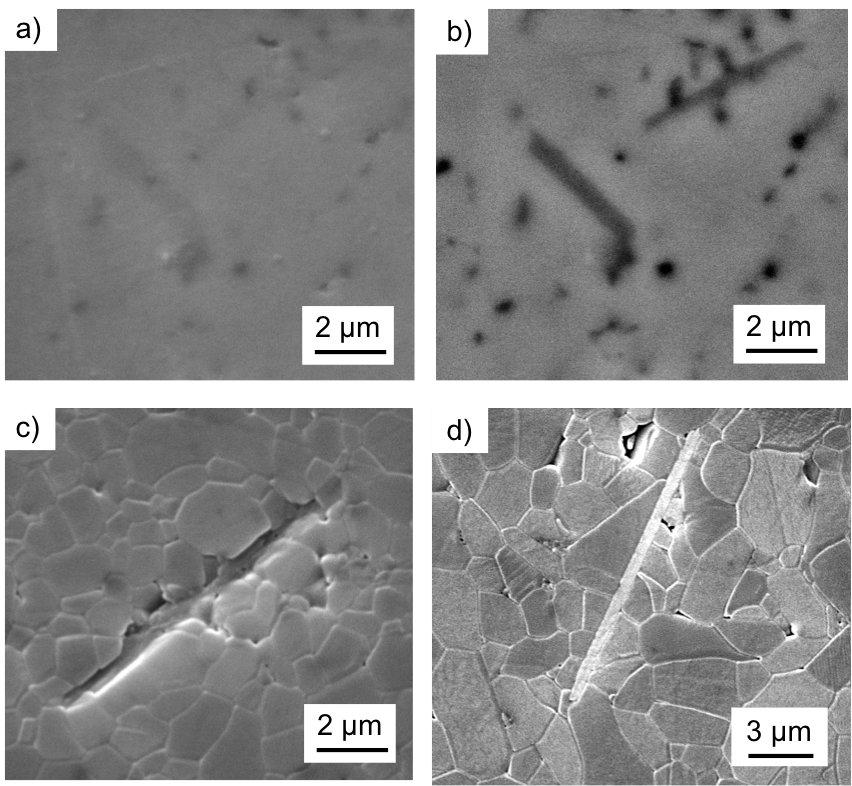
\includegraphics[width=\textwidth]{Chapter-5/Figures/Figure1.png}
	\caption{Micrographs of MgO-doped Bayer doped with 560 ppm Na$_{2}$O and 82 ppm SiO$_{2}$ after 3 h at 1525$^{\circ}$C obtained using a) a secondary electron detector and b) a backscattered electron detector.}
	\label{Ch5-figure:Figure1}
\end{figure}
%%%

\newpage
%%%
\begin{figure}[H]
	\centering
	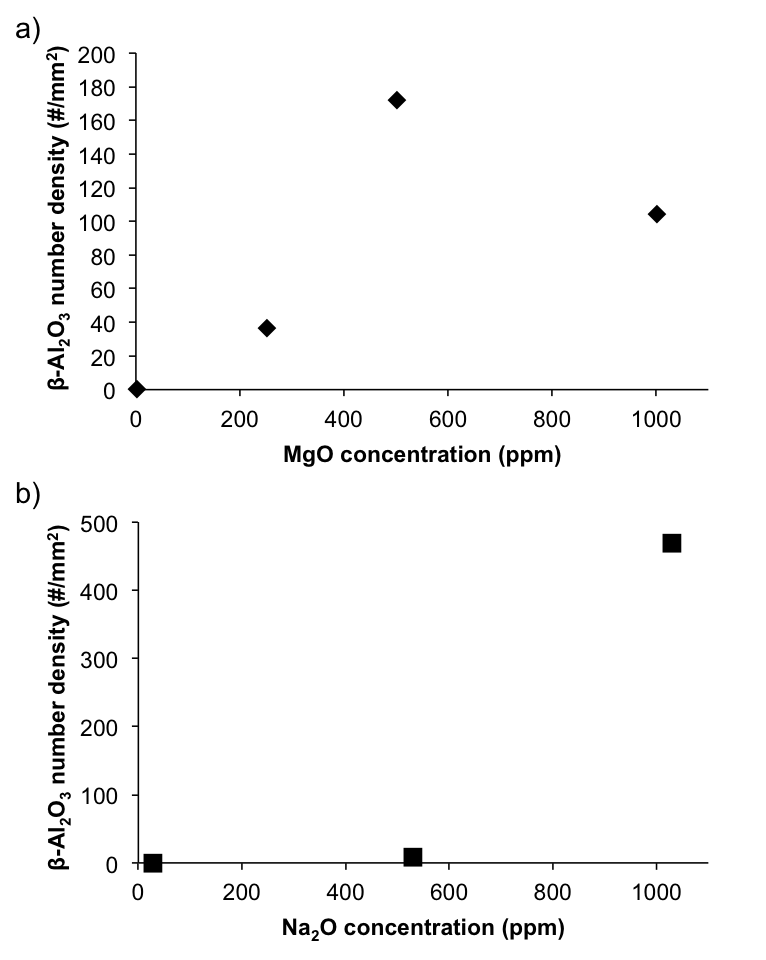
\includegraphics[scale=0.6]{Chapter-5/Figures/Figure2.png}
	\caption{a) XRD pattern and b) zoomed-in XRD pattern of a sample with 1060 ppm Na$_{2}$O, 82 ppm SiO$_{2}$, and 380 ppm MgO after sintering at 1525$^{\circ}$C for 5 h. All observed peaks except for one (*) can be assigned to either $\alpha$-Al$_{2}$O$_{3}$ or $\beta$-Al$_{2}$O$_{3}$.}
	\label{Ch5-figure:Figure2}
\end{figure}
%%%

\newpage
%%%
\begin{figure}[H]
	\centering
	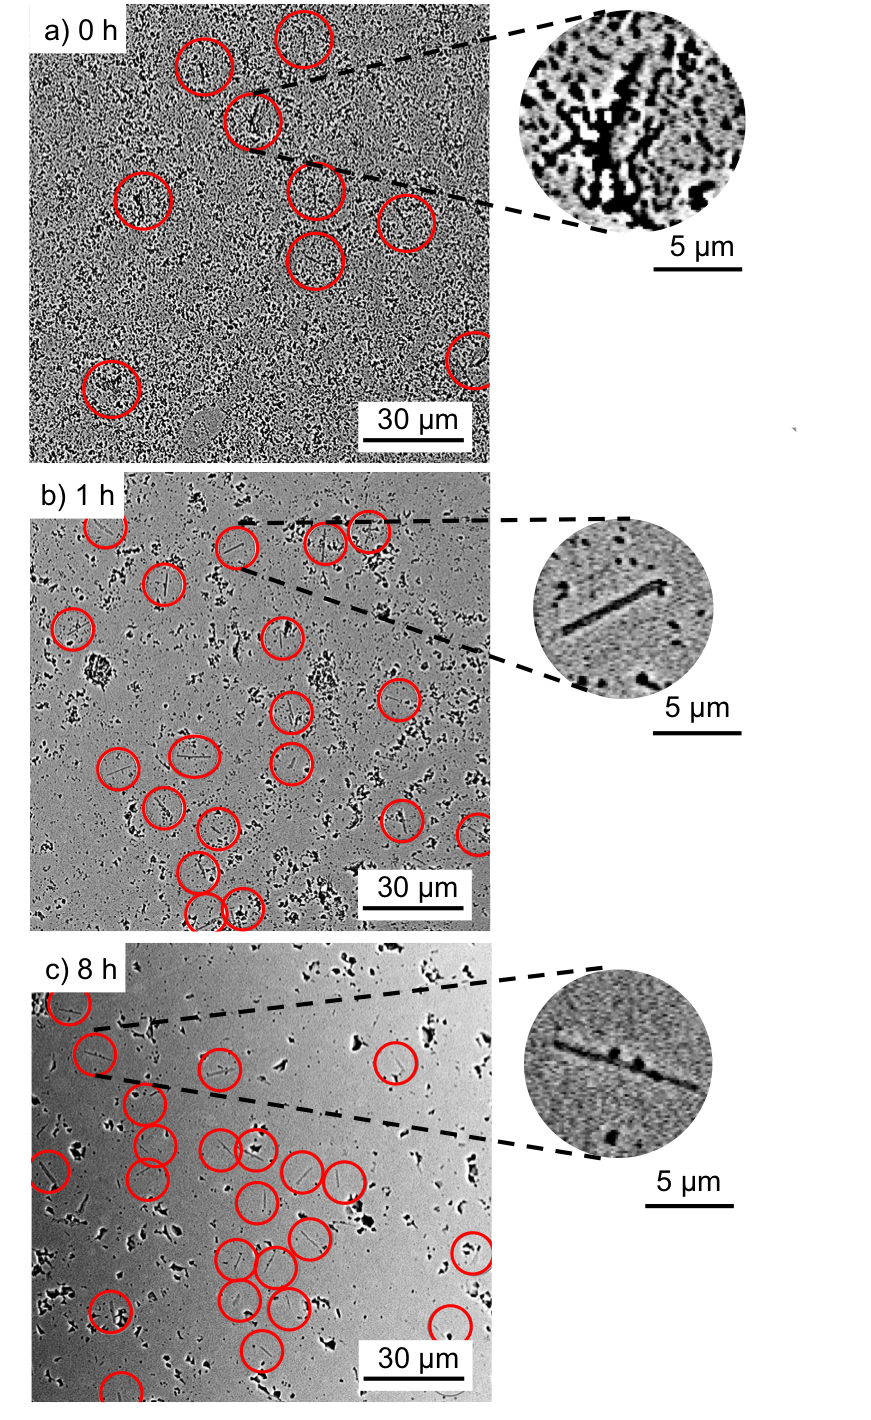
\includegraphics[scale=0.80]{Chapter-5/Figures/Figure3.png}
	\caption{Micrographs showing $\beta$-Al$_{2}$O$_{3}$ grains (red circles) in MgO-doped Bayer alumina samples with 82 ppm SiO$_{2}$ and 560 ppm Na$_{2}$O after sintering at 1525$^{\circ}$C for a) 0 h, b) 1 h, and c) 8 h.}
	\label{Ch5-figure:Figure3}
\end{figure}
%%%

\newpage
%%%
\begin{figure}[H]
	\centering
	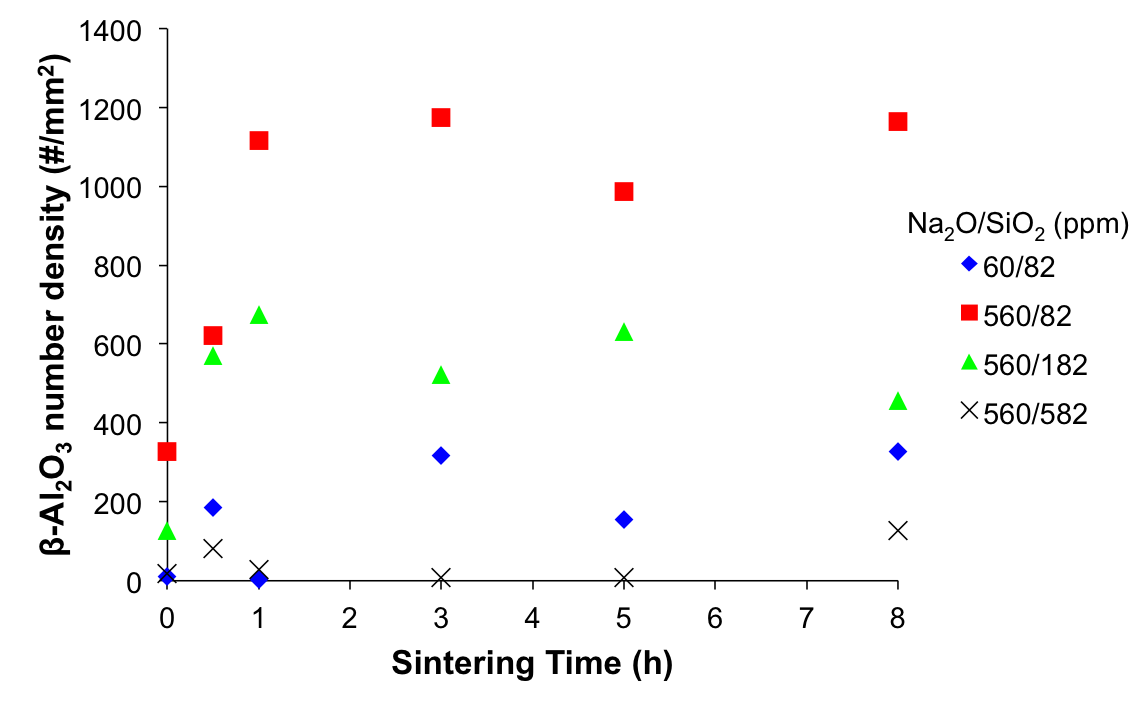
\includegraphics[width=\textwidth]{Chapter-5/Figures/Figure4.png}
	\caption{Kinetics of $\beta$-Al$_{2}$O$_{3}$ formation for different powder chemistries of MgO-doped powder samples.}
	\label{Ch5-figure:Figure4}
\end{figure}
%%%

\newpage
%%%
\begin{figure}[H]
	\centering
	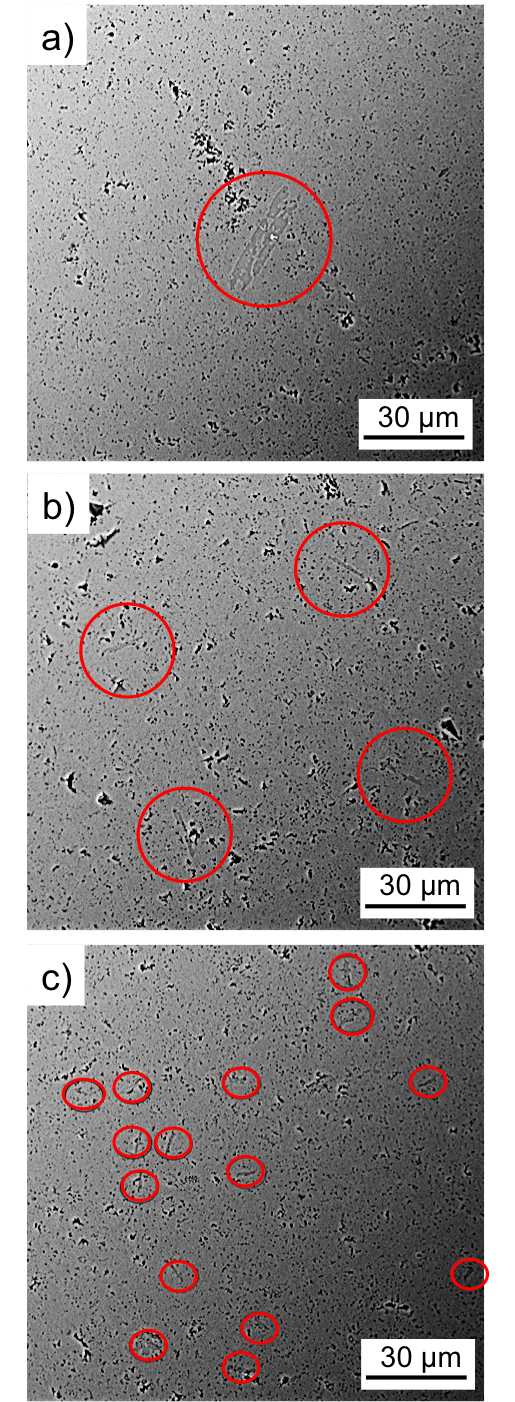
\includegraphics[scale=0.84]{Chapter-5/Figures/Figure5.png}
	\caption{Micrographs showing $\beta$-Al$_{2}$O$_{3}$ grains (red circles) in MgO-doped Bayer alumina samples with 82 ppm SiO$_{2}$ and a) 185 ppm Na$_{2}$O, b) 560 ppm Na$_{2}$O, and c) 1060 ppm Na$_{2}$O after sintering at 1525$^{\circ}$C for 3 h.}
	\label{Ch5-figure:Figure5}
\end{figure}
%%%

\newpage
%%%
\begin{figure}[H]
	\centering
	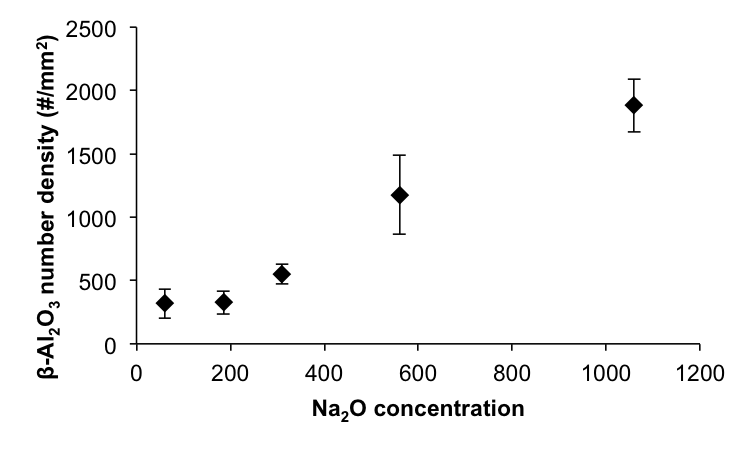
\includegraphics[scale=0.84]{Chapter-5/Figures/Figure6.png}
	\caption{Formation of $\beta$-Al$_{2}$O$_{3}$ a function of Na$_{2}$O concentration in MgO-doped Bayer alumina.}
	\label{Ch5-figure:Figure6}
\end{figure}
%%%

\newpage
%%%
\begin{figure}[H]
	\centering
	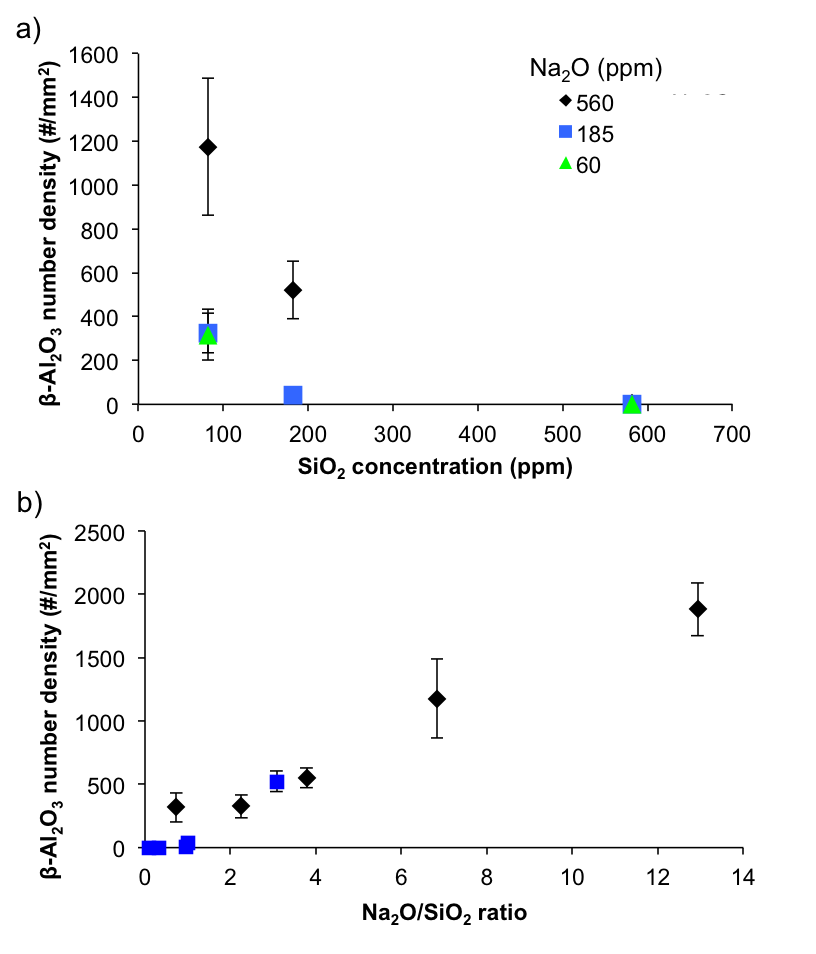
\includegraphics{Chapter-5/Figures/Figure7.png}
	\caption{Formation of $\beta$-Al$_{2}$O$_{3}$ in MgO-doped powder samples a function of a) SiO$_{2}$ concentration for different Na$_{2}$O concentrations, and b) Na$_{2}$O/SiO$_{2}$ ratio. In b) the black diamonds are samples with 82 ppm SiO$_{2}$ and the blue squares are samples with 182 and 582 ppm SiO$_{2}$.}
	\label{Ch5-figure:Figure7}
\end{figure}
%%%

\newpage
%%%
\begin{figure}[H]
	\centering
	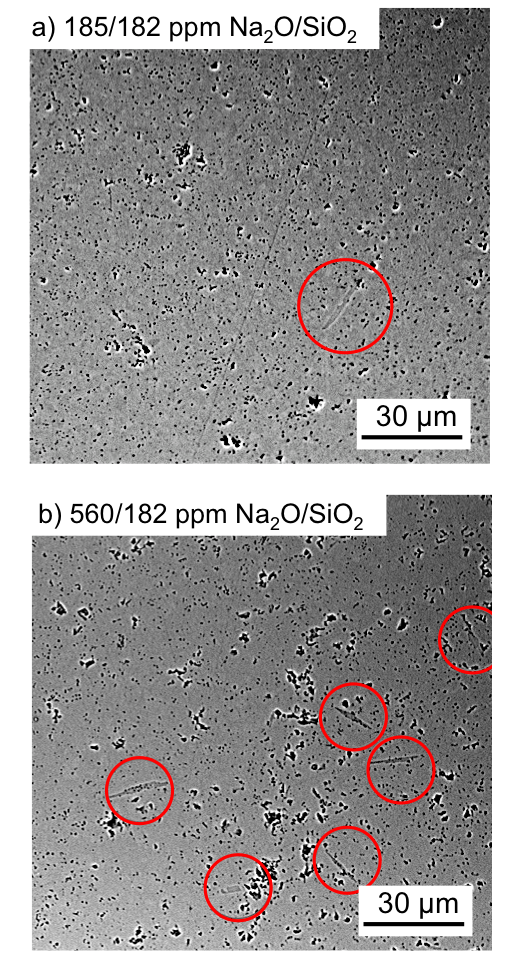
\includegraphics[scale=0.82]{Chapter-5/Figures/Figure8.png}
	\caption{Micrographs showing $\beta$-Al$_{2}$O$_{3}$ grains (red circles) in MgO-doped Bayer alumina samples with a) 185/182 ppm Na$_{2}$O/SiO$_{2}$ and b) 560/182 ppm Na$_{2}$O/SiO$_{2}$ after sintering at 1525$^{\circ}$C for 3 h.}
	\label{Ch5-figure:Figure8}
\end{figure}
%%%

\newpage
%%%
\begin{figure}[H]
	\centering
	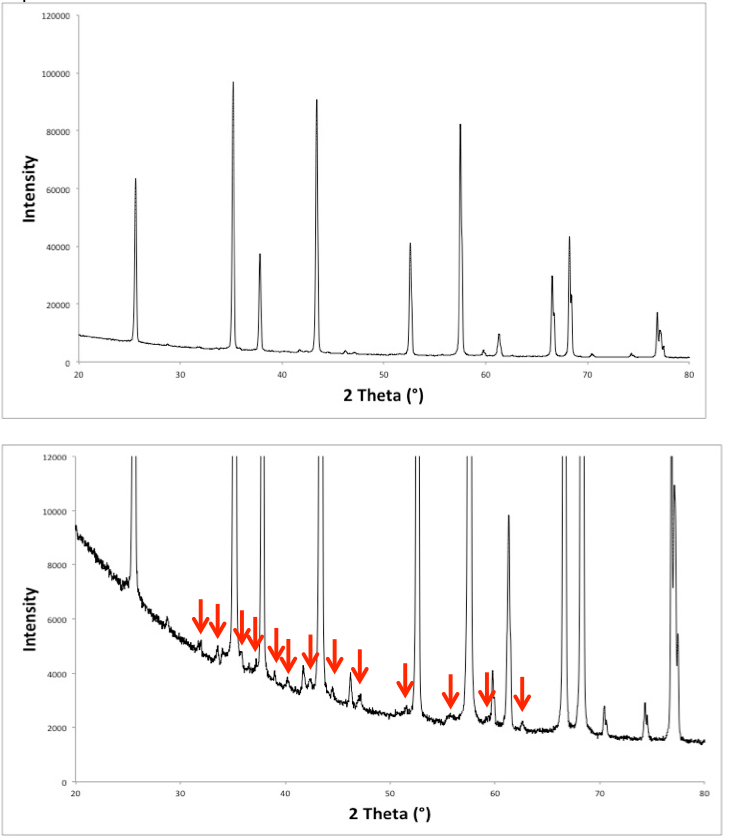
\includegraphics{Chapter-5/Figures/Figure9.png}
	\caption{Formation of $\beta$-Al$_{2}$O$_{3}$ in MgO-free powder samples as a function of a) MgO concentration (29 ppm Na$_{2}$O) and b) Na$_{2}$O concentration (2 ppm MgO) after 3 h at 1525$^{\circ}$C.}
	\label{Ch5-figure:Figure9}
\end{figure}
%%%

\newpage
%%%
\begin{figure}[H]
	\centering
	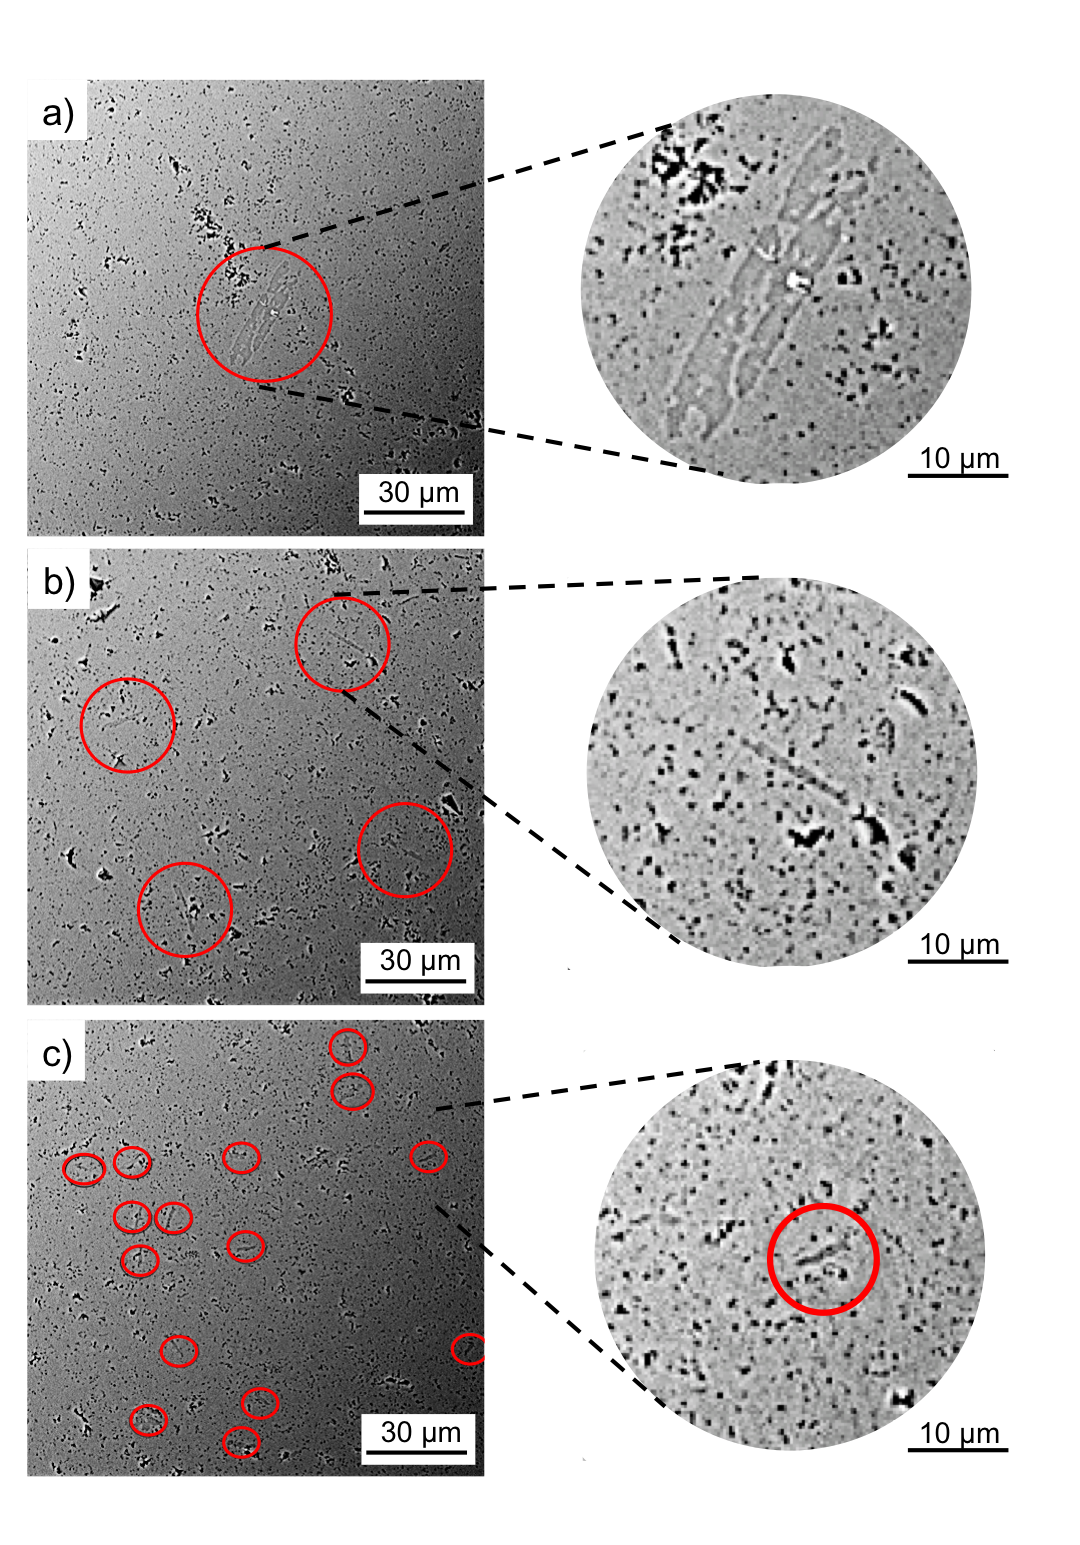
\includegraphics[scale=0.7]{Chapter-5/Figures/Figure10.png}
	\caption{Micrographs showing $\beta$-Al$_{2}$O$_{3}$ grains (red circles) in Bayer alumina samples with a) 1002 ppm MgO, 1000 ppm SiO$_{2}$, 29 ppm Na$_{2}$O, b) 2 ppm MgO, 1000 ppm SiO$_{2}$, 1029 ppm Na$_{2}$O, c) 1002 ppm MgO, 1000 ppm SiO$_{2}$, 1029 ppm Na$_{2}$O after 3 h at 1525$^{\circ}$C.}
	\label{Ch5-figure:Figure10}
\end{figure}
%%%

\newpage
%%%
\begin{figure}[H]
	\centering
	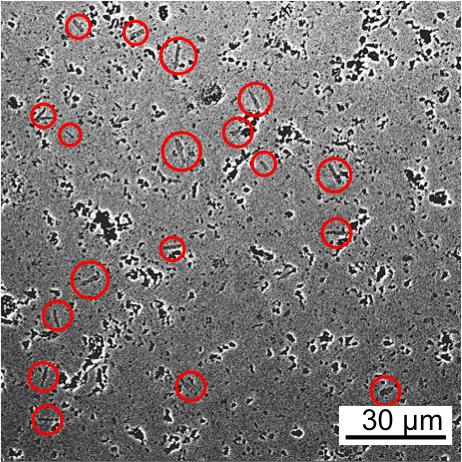
\includegraphics{Chapter-5/Figures/Figure11.png}
	\caption{Micrograph showing $\beta$-Al$_{2}$O$_{3}$ grains (red circles) in an ultra high purity powder sample with 502 ppm Na$_{2}$O, 2 ppm MgO, and 11 ppm SiO$_{2}$ after sintering at 1525$^{\circ}$C for 3 h.}
	\label{Ch5-figure:Figure11}
\end{figure}
%%%

